\section{Notions préliminaires}
	
	\subsection{Invariant de boucle}
		
		On appelle "invariant de boucle" une assertion mathématique qui est vraie à chaque tour de boucle. Lors de l'exécution d'un algorithme, on peut ainsi suivre son avancement via l'invariant de boucle.
		
		Cet invariant peut servir à démontrer la correction\footnote{la correction d'un algorithme est une preuve mathématique du fait que l'algorithme fait bien ce que l'on veut.} d'un algorithme en passant par une récurrence.
	
	\subsection{Complexité d'un algorithme}
		
		La complexité est une grandeur qui caractérise le nombre de calculs que l'algorithme demande. L'avantage de cette grandeur est qu'elle est propre à l'algorithme et n'est donc pas influencée par la machine qui exécute le programme.
		
		Pour déterminer la complexité, on compte le nombre d'opérations d'un certain type, choisi de manière à avoir une grandeur pertinente. On peut, par exemple, choisir de compter les comparaisons, les multiplications, les affectations de variables etc. La complexité doit s'exprimer en fonction de la taille des données d'entrées (la longueur d'une liste, le nombre de cases d'un tableau, le nombre de chiffres d'un nombre, etc.).

	\subsection{Terminaison d'un algorithme}
		
		Vérifier la terminaison d'un algorithme, c'est vérifier qu'il ne tournera pas indéfiniment.
		
		C'est généralement assez simple à prouver. On peut décomposer les preuves de terminaison d'algorithme en trois cas~:
		\begin{itemize}
			\item Les \python|for|~: le cas le plus simple, il y a un nombre fini de tour de boucle, il reste à s'assurer qu'aucune opération illicite n'est effectuée dans la boucle (pas de division par zéro, pas d'accès à un élément d'une liste qui n'existe pas ou qui est en dehors de la liste$\ldots$)
			\item Les \python|while|~: il faut s'assurer que la condition est fausse au bout d'un nombre fini de tour, cela peut s'avérer délicat, et l'on aura souvent recourt au point suivant. Il faut également vérifier qu'aucune opération illicite n'est effectuée.
			\item Le principe de descente infinie de Fermat~: toute suite d'entier positive et strictement décroissante atteint 0 au bout d'un temps fini.
		\end{itemize}

\section{Euclide~: Calcul du plus grand diviseur commun} \label{pgcd}
	
	\subsection{Principe}
	
		L'algorithme d'Euclide permet de calculer le plus grand diviseur commun entre deux entiers. Le principe repose sur la propriété du PGCD~: $PGCD(a~;\ b) = PGCD(b~;\ r)$ en notant $r$ le reste de la division euclidienne de $a$ par $b$, de plus $PGCD(a~;\ 0) = a$. Cette propriété du PGCD consistue l'invariant de boucle.
		
		L'invariant de boucle est ici~: $PGCD(a~;\ b) = PGCD(b~;\ r)$
	
	\subsection{Terminaison}
		
		En notant $a_n$ et $b_n$ les valeurs de $a$ et $b$ au $n^{\textrm{ième}}$ tour. Au début, nous avons~: $b_0 = b$. Et à chaque tour, $b_{n + 1} = a_n \ MOD\ b_n$. Or, par définition du reste de la division euclidienne, $a \ MOD\ b < b$.
		
		Ainsi $(b_n)_{n \in \mathbb{N}}$ est une suite positive et décroissante d'entiers, donc, d'après le principe de descente infinie de Fermat~:
		\[
			\exists N \in \mathbb{N},\ b_N = 0
		\]
		D'où la terminaison de l'algorithme.
		
	\subsection{Algorithme}
		
		\begin{pythoncode}
			def pgcd(a, b):
				# tant que b est non nul
				while b != 0:
					# a prend la valeur b
					# b prend pour valeur le reste de la division euclidienne de a par b
					a, b = b, a % b
				
				# b est nul, PDCG(a, 0) = a, on renvoie donc a
				return a
		\end{pythoncode}

\section{Bézout~: résolution d'équations diophantiennes}

	\subsection{Principe}
	
		Le principe de l'algorithme de Bézout est de résoudre des équations de la forme~: $au + bv = PGCD(a~;\ b)$. Aussi appelé "algorithme d'Euclide étendu", l'algorithme de Bézout calcule le plus grand diviseur commun à $a$ et $b$, ainsi qu'une paire de coefficients $(u~;\ v) \in \mathbb{Z}^2$.
		
		L'invariant de boucle est~:
		\[ \begin{array}{rcl}
			PGCD(r1~;\ r2) & = & PGCD(a~;\ b) \\
			r1 & = & au + bv \\
			r2 & = & as + bt
		\end{array} \]
	
	\subsection{Terminaison}
	
		La terminaison est la même que pour l'algorithme d'Euclide, avec $a = r1$ et $b = r2$.
	
	\subsection{Algorithme}
	
		\begin{pythoncode}
			def bezout(a, b):
				# on initialise les variables
				u, v, s, t = 1, 0, 0, 1
				r1, r2 = a, b
				
				# tant que b est non nul
				while r2 != 0:
					# q prend pour valeur le quotient de la division euclidienne de a par b
					q = r1 // r2
					r1, u, v = = r2, s, t
					r2 = r1 % r2
					s = u - q * s
					t = v - q * t
					
				# on retourne le PGCD ainsi que les coefficients (u; v)
				return r1, u, v
		\end{pythoncode}

\section{Dichotomie}

	Les algorithmes de dichotomies sont employés pour recherher un nombre dans une liste de nombres triés. Cette méthode à l'avantage d'avoir une très bonne complexité par rapport aux algorithmes de recherche qui parcourent la liste en entier.

	\subsection{Dans une liste triée}
		
		\subsubsection{Principe}
	
		On dispose d'une liste triée \python|ma_liste|, et on sait que si l'élément \python|element| que l'on cherche est dans la liste, alors il est dans la sous-liste \python|ma_liste[mini: maxi + 1]|.
		
		Au début on pose de l'algorithme~: \python|mini = 0| et \python|maxi = len(ma_liste) - 1|. En effet, si l'élément est dans la liste, alors il est dans la sous-liste \python|ma_liste[mini: maxi + 1]| (qui correspond alors à la liste entière).
		
		Au tour suivant, on calcule l'indice central de la liste~: \python|milieu = (mini + maxi) // 2|. Or la liste est triée, donc~:
		\begin{itemize}
			\item si \python|element > ma_liste[milieu]|, alors si l'élément est dans \python|ma_liste|, il est dans la sous-liste~: \python|ma_liste[milieu + 1: maxi]|
			\item si \python|element <= ma_liste[milieu]|, alors si l'élément est dans \python|ma_liste|, il est dans la sous-liste~: \python|ma_liste[mini: milieu]|
		\end{itemize} \ \\
		
		Cet algorithme a une complexité en $\Theta (\log n)$ où $n$ est la longueur de la liste donnée en argument.
		
		\subsubsection{Terminaison}
		
		Et tant que la condition \python|mini > maxi| est vraie on tourne. À chaque tour, l'écart \python|maxi - mini|, non seulement diminue, mais est divisé par deux. Donc le programme va donc nécessairement terminer (principe de descente inifinie de Fermat). Et à la fin, si l'élément est dans \python|ma_liste|, alors \python|element = ma_liste[mini]| (ou \python|element = ma_liste[maxi]|).
		
		\subsubsection{Algorithme}
		
		\begin{pythoncode}
			def dichotomie(ma_liste, element):
				# on initialize les variables
				mini = 0
				maxi = len(ma_liste) - 1
				
				while mini > maxi:
					# on calcule l'indice du milieu de la sous-liste
					milieu = (mini + maxi) // 2
					
					# on regarde dans quelle moitié de la sous-liste l'élément peut être
					if element > ma_liste[milieu]:
						mini = milieu + 1
					else:
						maxi = milieu
				
				return element == ma_liste[mini]
		\end{pythoncode}
	
	\subsection{Sur une fonction monotone}
		
		\subsubsection{Principe}
		
		De manière analogue à la précédente~; on cherche à trouver le point d'annulation d'une fonction monotone sur un intervalle $[mini~;\ maxi]$ avec une certaine précision.
		
		Comme pour la première version, on va calculer le milieu de l'intervalle et distinguer deux cas~:
		\begin{itemize}
			\item si $f(mini) \cdot f(milieu) > 0$~: $f(mini)$ et $f(milieu)$ sont donc de même signe or la fonction est monotone, donc le point d'annulation est après le milieu de l'intervale
			\item sinon, le points d'annulation est avant le milieu de l'intervalle
		\end{itemize} \ \\
		
		En comptant le nombre de tour de boucle, la complexité est un $\Theta (n)$ où $n$ est la précision (en bit) du résultat. Autrement dit, plus le résultat est précis, plus l'éxecution du programme sera longue.
		
		\subsubsection{Terminaison}
		
		En notant $a_n$ et $b_n$ les valeurs de $a$ et $b$ au $n^{\textrm{ième}}$ tour. Au sein d'un tour de boucle, on a~:
		\[
			\forall n \in \mathbb{N}^*,\ b_{n+1} - a_{n+1} = \frac{b_n - a_n}{2}
		\]
		
		Par récurrence, au bout de $k$ tours de boucle~:
		\[
			0 < b_k - a_k = \frac{b - a}{2^k}
		\]
		
		Or, $\frac{b - a}{2^k} \underset{k \to +\infty}{\longrightarrow} 0$ ainsi~:
		\[
			\forall \varepsilon > 0,\ \exists N \in \mathbb{N}^*,\ |b_N - a_N| < 2 \varepsilon
		\]
		
		\subsubsection{Algorithme}
			
		\begin{pythoncode}
			def dichotomie(f, mini, maxi, precision):
				while (maxi - mini) > 2 * precision:
					milieu = (maxi - mini) / 2
					if f(mini) * f(milieu) > 0:
						mini = milieu
					else:
						maxi = milieu
				return (maxi - mini) / 2
		\end{pythoncode}

\section{Méthode des rectangles et des trapèzes~: approximation d'une intégrale}
	
	\subsection{Principe}
		
		On considére une subdivision de l'intervalle sur lequel on veut approximer l'intégrale de $f$. Et pour chaque petit intervalle on va approximer la fonction par une fonction constante, ainsi, calculer l'aire sous la courbe va revenir à un calcul d'aire de rectangle (voir Figure~\ref{fig_3}).
		
		 On se place ainsi sur un segment $[a~;\ b]$ et on fixe un nombre arbitraire $n$ de subdivisions sur ce segment. Les largeurs des subdivisions sont égales\footnote{On parle alors de subdivision à pas constant.}, et valent~: $\frac{b - a}{n}$.
		 
		 La fonction étant approximée par une fonction constante, la hauteur du $k^{\textrm{ième}}$ rectangle vaut $f(a + k * largeur)$. Ainsi l'aire sous le $k^{\textrm{ième}}$ rectangle est de~: $\frac{b - a}{2} \cdot f \left( a + k \cdot \left( \frac{b - a}{2} \right) \right)$
		
		\begin{figure}[H]
			\centering
			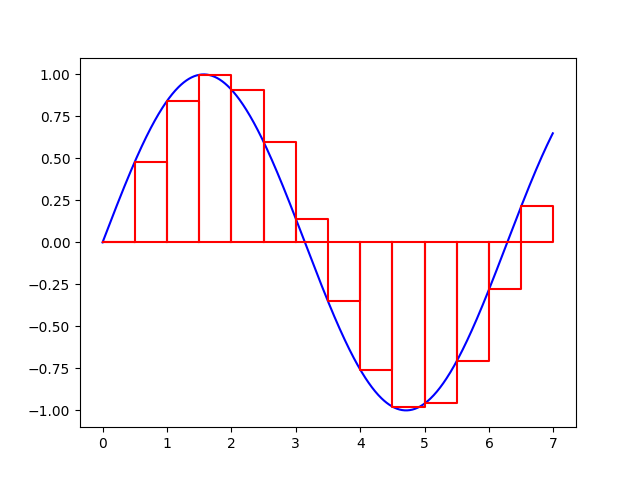
\includegraphics[scale=0.75]{images/Figure_3.png}
			\caption{Approximation de la fonction $sin$ avec un pas de 0.5}
			\label{fig_3}
		\end{figure}
	
	\subsection{Terminaison}
		
		Montrer la terminaison ne pose pas de problème~: l'algorithme repose sur une boucle itérative finie et aucune opération illicite n'est effectuée.
	
	\subsection{Algorithme}
	
		\begin{pythoncode}
			def rectangle(f, a, b, n):
				# l'aire vaut zéro au début
				integrale = 0
				
				# le pas étant constant, la largeur est la même partout
				largeur = (b - a) / n
				
				for k in range(n):
					# on calcule la hauteur
					hauteur = f(a + k * largeur)
					
					# on ajoute l'aire du rectangle à l'intérgrale
					integrale += hauteur * largeur
				
				# on renvoie la somme des aires des rectangles
				return integrale	
		\end{pythoncode}
	
	\subsection{Méthode des trapèzes}
		
		La méthode est sensiblement la même, mais on approxime la fonction par des fonctions affines et non plus des constantes.
		
		\begin{figure}[htp]
			\centering
			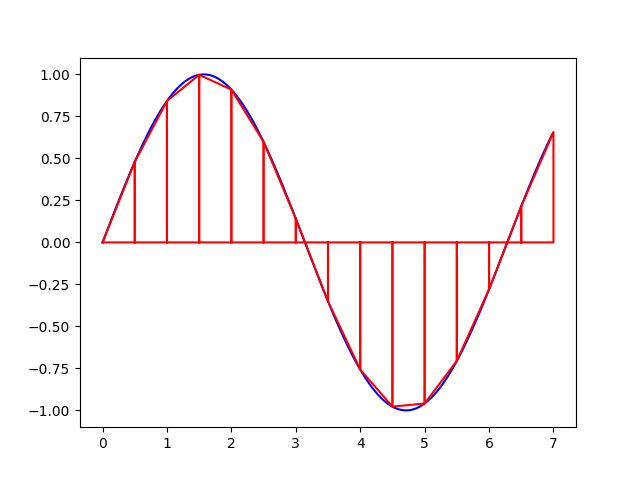
\includegraphics[scale=0.75]{images/Figure_4.png}
			\caption{Approximation de la fonction $sin$ avec un pas de 0.5}
		\end{figure}
		
		La largeur ne change pas par rapport à la méthode des rectangles, mais la hauteur devient la moyenne entre $f(a + k * largeur)$ et $f(a + (k + 1) * largeur)$. Ainsi~:
		
		\begin{pythoncode}
			def trapeze(f, a, b, n):
				integrale = 0
				largeur = (b - a) / n
				
				for k in range(n):
					hauteur = f(a + k * largeur) + f(a + (k+1) * largeur)
					integrale += largeur * hauteur / 2
				
				return integrale
		\end{pythoncode}

\section{Méthode d'Euler~: résolution d'une équation différentielle}
	
	\subsection{Principe}
		
		Cette méthode permet de résoudre des équations différentielles d'ordre 1 de la forme~:
		\[
			\forall t \in [a~;\ b],\ y'(t) = f(t, y(t))
		\]
		dans lesquelles on cherche $y$.
		
		On considère les conditions initiales~: $(t_0~;\ y_0)$ telles que $y_0 = y(t_0)$, et un intervalle $[0~;\ T]$ dans lequel va varier $t$. L'enjeu est de prendre des valeurs suffisamment proches tout en conservant un temps de calcul raisonnable, à l'instar de la méthode des rectangles, nous allons subdiviser l'intervalle $[a~;\ b]$ en $N$ sous-intervalles de longeur~: $h = \frac{b - a}{N}$\footnote{$h$ est le pas et l'on a~: $t_{n+1} = t_n + h$}. On définit alors les valeurs de $t_n$ pour lesquelles on va approximer $y(t_n)$ par $y_n$~:
		\[
			\forall n \in \llbracket 0~;\ N \rrbracket,\ t_n = nh
		\]
		
		Ainsi, nous allons avoir une suite $(y_n)_{n \in \llbracket 0~;\ N \rrbracket}$ et~:
		\[
			 \forall n \in \llbracket 0~;\ N \rrbracket,\ y_n \approx y(t_n)
		\]
		
		Les $y_n$ sont calculables de proche en proche grâce à la formule de récurrence~:
		\[
			\forall n \in \llbracket 0~;\ N \rrbracket,\ y_{n+1} = y_n + h \cdot f(t, y_n)
		\]
		
		Il restera enfin à tracer la courbe des $y_n$ (voir chapitre~\ref{chap_4}).
	
	\subsection{Terminaison}
		
		Comme pour la méthode des rectangles, il n'y a qu'une boucle for, ni aucune opération illicite, donc le programme termine.
		
	\subsection{Algorithme}
		
		Avec des listes Python~:
		\begin{pythoncode}
			def euler(f, a, b, N, y0):
				# on calcule le pas
				h = (b - a) / N
				
				# construction des abscisses
				X = [a + n * h for n in range(N)]
				
				# on simplifie un peu le problème en considérant y(a) = y0
				Y = [y0]
				
				# N - 1 car la première valeur (condition initiale) est déjà dans la liste
				for i in range(N - 1):
					# on extrait le tn et yn
					t, y = X[i], Y[i]
					
					# calcul de y_{n+1}
					y = y + h * f(t, y)
					
					# on stocke la nouvelle valeur de y (y_{n+1})
					Y.append(y)
				
				# on renvoie les points calculés (pour tracer une courbe par exemple)
				return X, Y
		\end{pythoncode}
		On peut tout à fait raccourcir la boucle \python|for| en~:
		\begin{pythoncode}
			for i in range(N - 1):
				Y.append(Y[i] + h * f(X[i], Y[i]))
		\end{pythoncode}
		
		Avec des \python|array| (voir~\ref{numpy})~:
		\begin{pythoncode}
			def euler(f, a, b, N, y0):		
				X = np.linspace(a, b, N)
				Y = np.zeros(N)
				
				# condition initiale y(a) = y0
				Y[0] = y0
				
				# calcul du pas
				h = (b - a) / N
				
				# calcul des abcisses
				for i in range(N):
					Y[i + 1] = Y[i] + h * f(X[i], Y[i])
				
				return X, Y
		\end{pythoncode}
	
	\subsection{Application} \label{appl:equa_diff} (Corrigé~: \ref{corr:equa_diff})
		
		On cherche à résoudre l'équation différentielle~:
		\[
			\forall t \in [-1~;\ 10],\ (t^2 + 1)y' + (t - 1)^2y = t^3 - t^2 + t + 1
		\]
		Avec la condition initiale~: $y(-1) = 8$.
		Le but est de reprogrammer l'algorithme, pas d'utiliser les fonctions.
		
		Les grandes étapes~:
		\begin{enumerate}
			\item Il faut commencer par isoler $y'$ pour trouver $f$, une fonction de $t$ et de $y$.
			\item Construire le tableau des ordonnées.
			\item Construire les abcisses de la solution pour une condition initiale donnée.
			\item Tracer la courbe de la solution.
			\item (Juste parce que c'est joli, recommencer avec une autre condition initiale.)
		\end{enumerate}

\section{Exponentiation rapide}
	
	\subsection{Principe}
		
		Dans toute cette sous-section, nous voulons élever $x \in \mathbb{R}$ à une puissance $p \in \mathbb{N}^*$. Partons de l'algorithme naïf, récursif d'exponentiation~:
		\begin{pythoncode}
			def puissance(x, p):
				if p == 0: return 1
				else: return x * puissance(x, p - 1)
		\end{pythoncode}
		
		Ainsi, cet algorithme va effectuer $p$ tours de boucles avant de terminer. Sa complexité est donc un $\Theta(p)$. Cette complexité n'est pas catastrophique, mais on peut mieux faire. Pour cela il faut remarquer trois choses~:
		\begin{itemize}
			\item si $p = 0$, $x^p = 1$
			\item si $p$ est pair, $x^p = (x^2)^{\frac{p}{2}}$
			\item si $p$ est impair, $x^p = x \times (x^2)^{\frac{p - 1}{2}}$
		\end{itemize}
		
		Ainsi, si $p$ est pair, on peut calculer $y^{\frac{p}{2}}$ avec $y = x^2$, si $p$ est impair, on calcule $y^{\frac{p - 1}{2}}$ avec $y = x^2$ et on multiplie par $x$.
		
		La différence peut sembler futile, mais si on représente le nombre de multiplication effectuées pour calculer les puissances de 5 de 1 à 100~:
		\begin{figure}[htp]
			\centering
			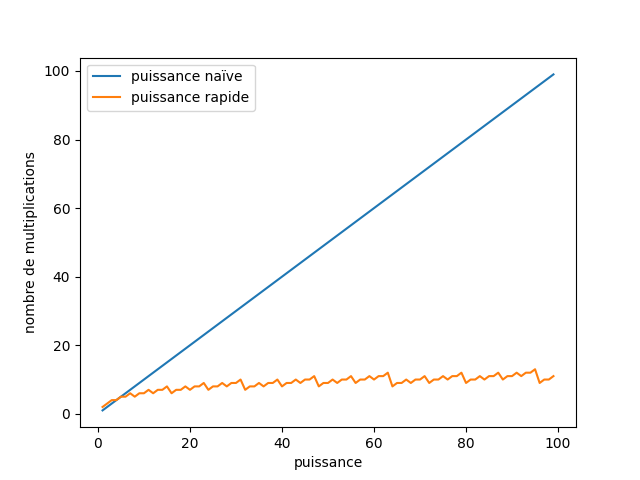
\includegraphics[scale=0.75]{images/Figure_7.png}
			\caption{Nombre de multiplications effectuées en fonctions de la puissance}
		\end{figure}
		On se rend compte que l'algorithme rapide est réellement plus performant que l'algorithme naïf. De plus, on peut montrer par le calcul que l'exponentiation rapide a une complexité en $\Theta (\log n)$.
		
	\subsection{Terminaison}
		
		L'algorithme termine car $p$ est un entier postif, qui décroît à chaque tour de boucle (il est divisé par deux à chaque fois). Donc d'après le principe de descente infinie de Fermat, $p$ va finir par être nul.
	
	\subsection{Algorithme}
		On peut écrire une version récursive~:
		\begin{pythoncode}
			def puissance_rapide(x, p):
				if p == 0: return 1
				elif p % 2: return x * puissance(x**2, (p - 1) // 2) # si p % 2 != 0 donc si p est impair
				else: return puissance(x**2, p // 2)
		\end{pythoncode}


\section{Binaire et changement de bases}

	\subsection{Principe}
		
		Dans les ordinateurs, les nombres sont représentés par une représentation dite en "binaire". Il s'agit d'une succession de 0 et de 1 qui correspondent au nombre. De manière courante nous utilisons la notation en base 10. L'enjeux de cette partie est de voir comment baser du binaire au décimal et d'implémenter cet algorithme. Dans la représentation binaire, on appelle nombre de bits le nombre de chiffres. Quelques exemples sur deux bits~: \\
		\begin{tabular}{|l|l|} \hline
			décimal & binaire \\ \hline
			0 & 00 \\ \hline
			1 & 01 \\ \hline
			2 & 10 \\ \hline
			3 & 11 \\ \hline
		\end{tabular} \\

		Pour passer du binaire au décimal, il faut écrire chaque chiffre du nombre ainsi que la puissance de 2 auquel il est associé. La méthode générale est de partir du chiffre le plus à gauche et de lui associé la puissance $2^0$, le chiffre juste à droite reçoit reçoit la puissance $2^1$ et ainsi de suite. Par exemple, si l'on prend le nombre écrit en binaire $1011$~:
		\[ \begin{array}{llll}
			2^3 & 2^2 & 2^1 & 2^0 \\
			1   & 0   & 1   & 1 \\
		\end{array} \]
		
		Ainsi $1011$ en binaire, peut se décomposer en décimal comme $1 \times 2^3 + 0 \times 2^2 + 1 \times 2^1 + 1 \times 2^0$, d'où~:
		\[ \begin{array}{rcl}
			1 \times 2^3 + 0 \times 2^2 + 1 \times 2^1 + 1 \times 2^0 & = & 1 \times 8 + 0 \times 4 + 1 \times 2 + 1 \times 1 \\
			& = & 8 + 2 + 1 \\
			& = & 11
		\end{array} \]
		Ainsi le nombre $1011$ en binaire est équivalent au nombre $11$ en décimal. \\
		
		Pour passer du décimal au binaire, il faut décomposer le nombre en décimal en effectuant des disivions euclidiennes par deux et en gardant les restes tant que le quotient est non nul. Reprenons $11$ comme point de départ.
		\begin{itemize}
			\item on divise $11$ par $2$. $11 = 2 \times 5 + 1$, on garde le $1$
			\item $5 = 2 \times 2 + 1$, on place ce deuxième reste ($1$) à droite du premier. (le nombre décomposé en binaire ressemble alors à~: $..11$).
			\item $2 = 2 \times 1 + 0$ donc on met le $0$ à droite des deux premiers chiffres et on continue car $1$ est non nul
			\item $1 = 2 \times 0 + 1$ on place alors ce dernier reste à droite des trois premiers chiffres et on s'arrête car le quotient est nul.
		\end{itemize}
		
		On retrouve alors le nombre $1011$ en binaire.

	\subsection{Terminaison}
		
		Dans le cas du passage du binaire vers le décimal, l'algorithme va devoir parcourir tous les chiffres du nombre, la boucle \python|for| ne contenant pas d'opérations illicites, l'algorithme est fini.
		
		Pour le cas de la conversion, l'algorithme boucle tant que le quotient est non nul, or le quotient est divisé par deux au tour suivant. Ainsi la suite des quotients au fil des tours de boucle forme une suite d'entiers positifs décroissantes, donc il existe un quotient nul, d'où la terminaison de l'algorithme.
	
	\subsection{Algorithme}
		
		Pour passer du binaire au décimale, la fonction va prendre en argument le nombre au format binaire dans une chaîne de caractère et appliquer le principe vu plus haut, de manière à renvoyer un entier en base 10.
		\begin{pythoncode}
			def decimal(nb_binaire):
				resultat = 0
				for i in range(len(nb_binaire)):
					chiffre = int(nb_binaire[-(i + 1)] # on extrait le chiffre d'indice i en partant de la fin
					puissance_deux = 2 ** i # on calcule la puissance de 2 correspondante
					resultat += chiffre * puissance_deux # on ajoute au résultat
				return resultat
		\end{pythoncode}
		
		Pour convertir un nombre du format décimal vers le binaire, nous allons faire une fonction qui va prendre en argument le nombre à convertir et qui va renvoyer la liste des chiffres en binaire.
		\begin{pythoncode}
			def binaire(nb_decimal):
				resultat = [nb_decimal % 2] # on initialise la liste avec le premier reste
				nb_decimal //= 2 # on divise le nombre pour garder le quotient
				while nb_decimal: # tant que le quotient est non nul
					resultat.insert(0, nb_decimal % 2) # on insert à droite du premier élément, le reste suivant
					nb_decimal //= 2 # on calcule le quotient suivant
				return resultat # on renvoie la liste des restes
		\end{pythoncode}

\section{Tri par insertion}
	
	\subsection{Principe}
		
		Le principe est de parcourir la liste, et tant que l'élément que l'on regarde est plus petit que l'élément précédent et que les indices sont positifs, on inverse les éléments.\\
		
		En prenant $n$, la longueur de la liste, la complexité est en $\Theta(n)$ si la liste est déjà triée (complexité dans le meilleur cas), et peut atteindre $\Theta(n^2)$ dans le pire cas.
		
	\subsection{Terminaison}
		
		La boucle \python|while| termine car soit l'élément que l'on déplace est décalé jusqu'à la première case de la liste, soit l'élément se retrouve à sa place. La boucle \python|for| termine car on ne parcourt la liste qu'une seule fois.
	
	\subsection{Algorithme}

		\begin{pythoncode}
			def tri_insertion(liste):
				for i in range(1, len(liste)):
					element_a_trier = liste[i]
					j = i
					while j > 0 and element_a_trier < liste[j - 1]: # tant que 'element_a_trier' n'est pas à sa place et que l'indice est positif
						liste[j] = liste[j - 1] # on recule l'élément à trier dans la liste
						j -= 1 # on recule l'indice de l'élément comparé
					liste[j] = element_a_trier # on insert l'élément à trier à sa place
		\end{pythoncode}
		
\section{Tri-fusion}
	
	\subsection{Principe}
		
		Le tri fusion repose sur un principe simple~:
		\begin{itemize}
			\item une liste a un seul élément est triée
			\item pour trier une liste à $n$ éléments on fusionne les deux sous-listes de longeurs égales extraites de cette liste
		\end{itemize}
		
		On va donc commencer par diviser la liste donnée en argument en plusieurs sous-listes jusqu'à obtenir des listes de longueur 1. On triera ensuite les listes en les fusionnant. \\
		
		Le fonctionnement de la fusion est central. On note $a$ et $b$ les deux sous-listes à fusionner et $a_i$ et $b_i$ les $i^{\textrm{ième}}$ éléments des listes $a$ et $b$. On prend un indice $i$ associé à la liste $a$ et un indice $j$ associé à $b$. 
		
		On initialise $i$ et $j$ à $0$, et on créée une liste vide $c$ munie d'un indice $k$ initialisé à $0$ aussi.
		
		Tant que $i$ est inférieur à la taille de $a$ et $j$ est inférieur à la taille de $b$, on boucle suivant le principe suivant~:
		\begin{itemize}
			\item si $a_i \leq b_j$, on ajoute $a_i$ à $c$, on incrémente $i$ de un
			\item si $a_i > b_k$, on ajoute $b_j$ à la liste $c$, et on incrémente $j$ de un
		\end{itemize}
		La liste $c$ est alors la liste triée résultant de la fusion entre $a$ et $b$. \\
		
		La complexité du tri-fusion dans le pire cas se divise en trois parties~: le tri de la première sous-liste, de la seconde sous-liste, et la fusion des deux. On peut alors montrer que si la liste donnée est de taille $n$ la complexité est en $\Theta(n \log n)$.
		
	\subsection{Terminaison}
	
		L'algorithme de fusion est terminé, puisqu'à chaque tour, soit $i$ soit $j$ augmente d'un, donc on finit par atteindre la taille des sous-listes.
		e
		La fonction principale va découper la liste en sous-liste de longeur $\frac{n}{2}$ à chaque tour, donc on finira par avoir des listes de longueurs un qui sont, par définition, déjà triées.
		
	\subsection{Algorithme}
		
		\begin{pythoncode}
			def fusion(a, b):
				i = j = 0
				c = []
				while i < len(a) or j < len(j):
					if j == len(b) or (i < len(a) and a[i] <= b[j]):
						c.append(a[i])
						i += 1
					elif i == len(a) or (j < len(b) and a[i] > b[j]):
						c.append(b[j])
						j += 1
				return c
			
			def tri_fusion(liste):
				n = len(liste)
				if n == 1: return liste
				else: return fusion(tri(liste[n // 2: ]), tri(liste[: n // 2]))
		\end{pythoncode}
			
			
				
